

\section{Frontend Development}

\subsection{UI/UX Design Using Figma}
The design of the user interface was initially conceptualized on Figma, focusing on user experience and intuitive navigation. The goal was to create a streamlined interface for laboratory personnel to monitor equipment and data efficiently.

\begin{figure}[H]
    \centering
    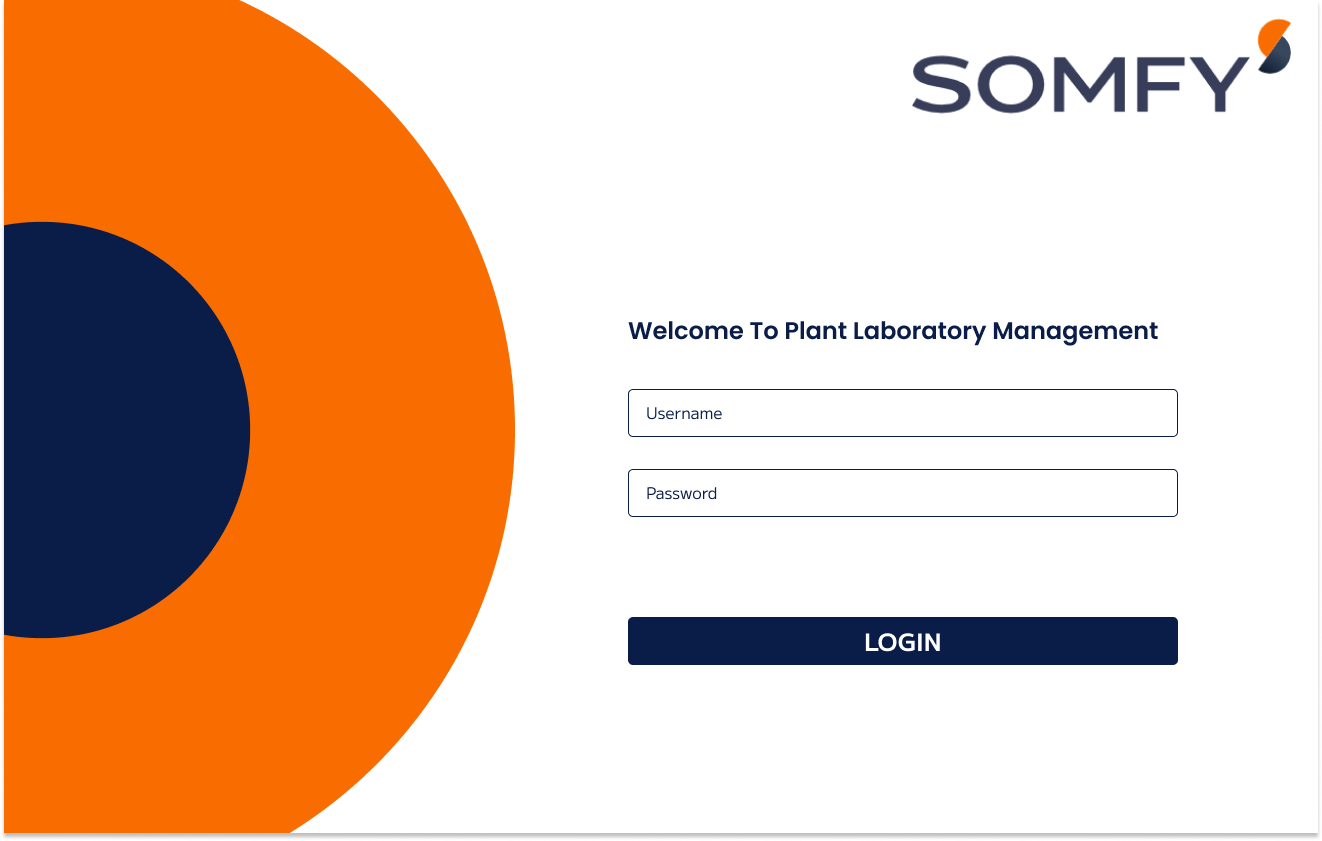
\includegraphics[width=1\textwidth]{chapters/3/img/10.png}
    \caption{cp 242-1 LEAN}
    \label{fig:campus}
\end{figure}

BLABALALALALNA LNNNLLALD

\begin{figure}[H]
    \centering
    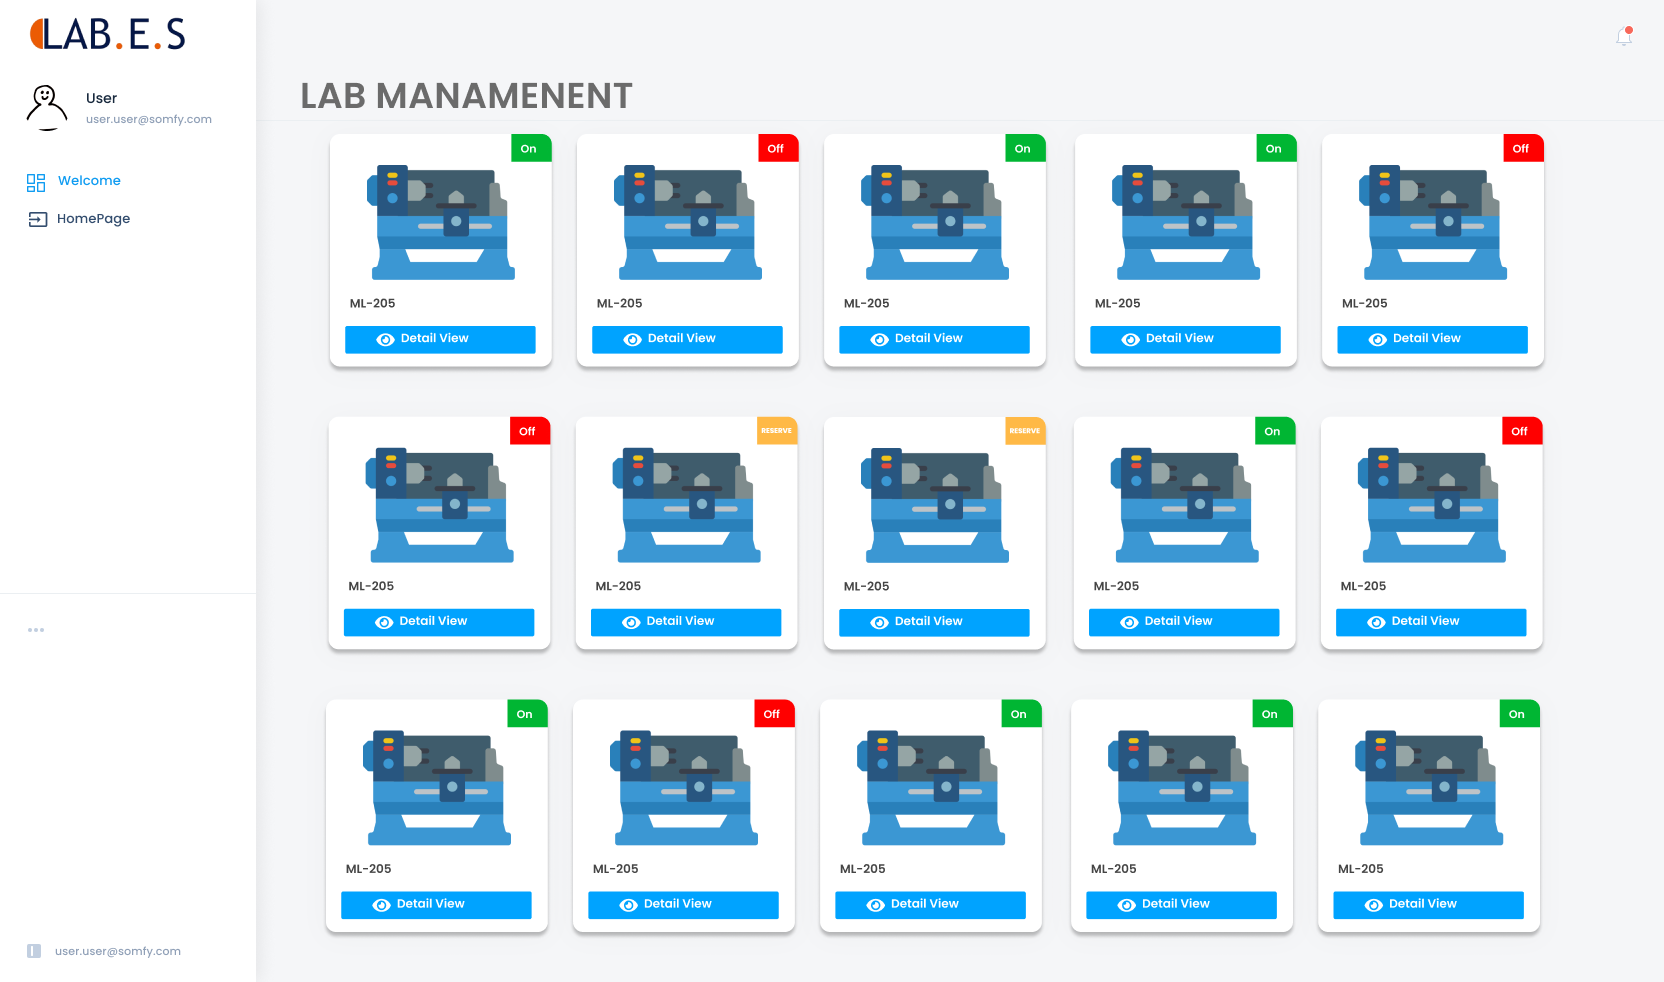
\includegraphics[width=1\textwidth]{chapters/3/img/12.png}
    \caption{cp 242-1 LEAN}
    \label{fig:campus}
\end{figure}



\subsection{ReactJS Implementation}
The frontend was implemented using ReactJS, leveraging its component-based architecture. This allowed for the creation of reusable components, reducing development time. Key features include:
\begin{itemize}
    \item \textbf{Real-Time Data Visualization}: Dynamic dashboards to monitor lab operations.
    \item \textbf{Interactive Forms}: Efficient data entry and equipment management.
    \item \textbf{Responsive Design}: Ensuring compatibility across devices, from desktops to tablets.
\end{itemize}


\begin{figure}[H]
    \centering
    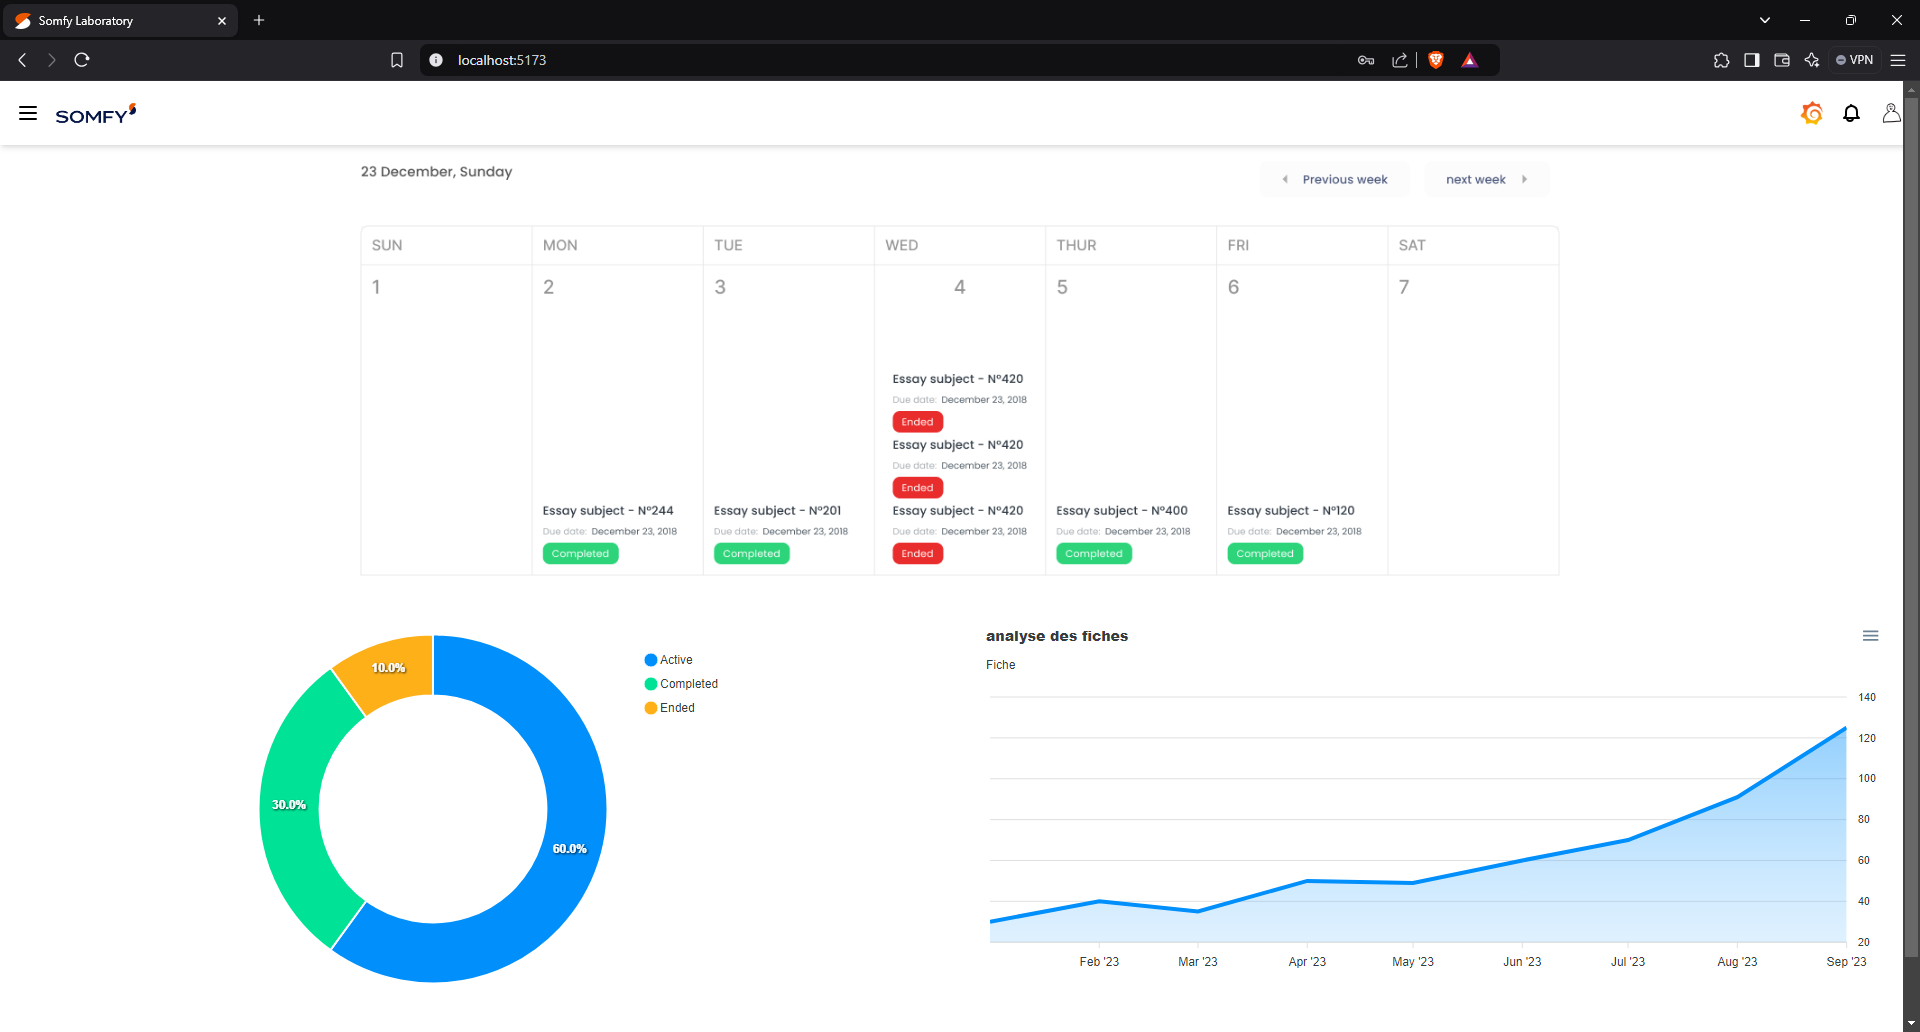
\includegraphics[width=1\textwidth]{chapters/3/img/2.png}
    \caption{cp 242-1 LEAN}
    \label{fig:campus}
\end{figure}


\begin{figure}[H]
    \centering
    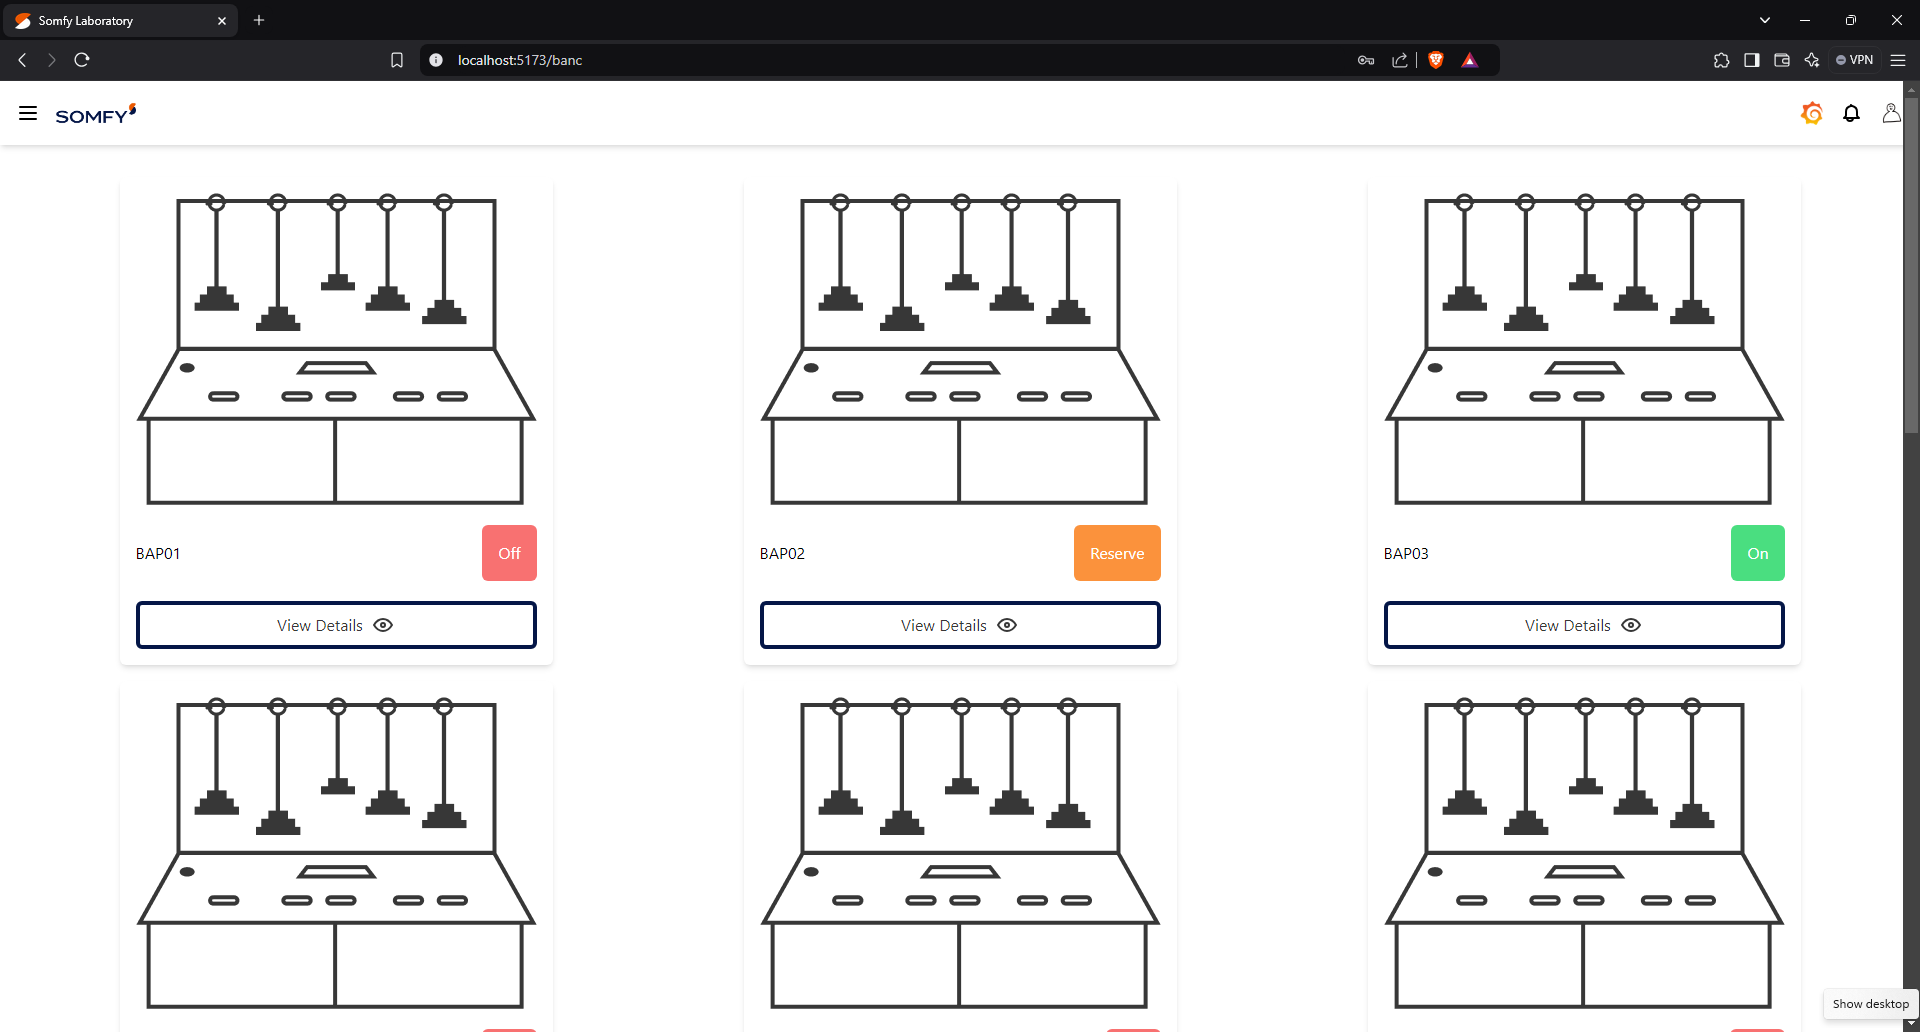
\includegraphics[width=1\textwidth]{chapters/3/img/6.png}
    \caption{cp 242-1 LEAN}
    \label{fig:campus}
\end{figure}








